\chapter{Background}
\label{chap:hardware}

    \section{Hardware Description}
    \label{sec:hardware-description}
        %% TODO
        %% Target models of computation: register machine x boolean circuits
        %%     trade-off in complexity (size x cycles)
        %% General trend to raise the level of abstraction of descriptions
        %% Hardware description languages
        %% Attempts at High-Level Synthesis and so forth (TCC)

        The hardware development process can be well understood by analyzing its
        similarities and differences to software development.
        Both hardware and software development usually "begin" with a high-level \emph{specification}
        of the algorithm to be implemented.
        Also, both proceed by a series of translations, increasingly adding more details to the description.

        However, the final targets of both hardware and software development differ:
        while in software the final artifact is machine code (sequence of instructions) for some architecture,
        in hardware the target is usually a \emph{floorplan}, a spacially placed graph of logic gates and wires.
        Also, the transformation steps in the software and hardware chains are different,
        as depicted in figure~\ref{fig:sw-hw-chains}.

        \begin{figure}[h]
            \centerline{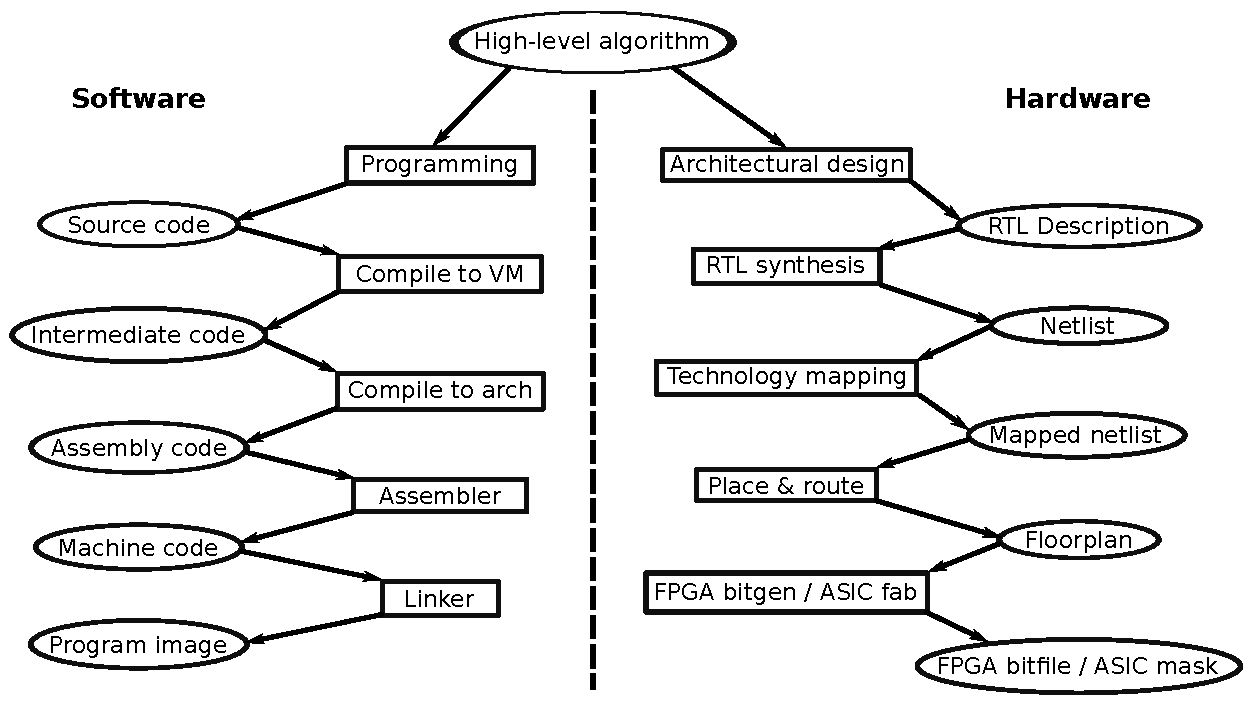
\includegraphics[width=0.9\textwidth]{imgs/sw-hw-chains.pdf}}
            \caption{Software and Hardware refinement chains. \label{fig:sw-hw-chains}}
        \end{figure}

        \acrodef{HDL}{Hardware Description Language}
        \acrodef{RTL}{Register-Transfer Level}
        The first (higher) levels in the hardware implementation flow is usually described using
        so-called \acp{HDL}, most popularly Verilog and \acs{VHDL}.
        %% Mention usage both for behavioural AND RTL.
        However, these languages were originally designed for \emph{simulation} purposes,
        and there are several problems that arise when using them to model hardware
        \emph{architecture} at \ac{RTL}.

        First of all, only a \emph{subset} of these languages can be used for \emph{synthesis}
        (actually deriving a netlist and floorplan).
        Although there is a standard defining a \emph{synthesizable subset} of \acs{VHDL}~\cite{ieee1076-3-synth-vhdl},
        tools differ greatly in the level of support.
        To further complicate the matter, this synthesizable subset is not syntactically seggregated.
        One example of complex requirement for \acs{VHDL} to be synthesizable is:
        "in a process, every output must be assigned a value for every possible combination of input values".
        In listing~\ref{lst:vhdl-unsynth-process} we have a process which violates this requirement.

        \begin{listing}[h]
            \begin{center}
                \vhdlfile{code/vhdl-unsynth-process.vhd}
            \end{center}
            \caption{Unsynthesizable \acs{VHDL} process \label{lst:vhdl-unsynth-process}}
        \end{listing}

        % TODO: go on... Mention HLS, verification efforts, etc, but having synthesizable
        % model AND proof in the same language is a nicer framework


    \section{Functional Hardware Description}
    \label{sec:functional-hardware}
        In the beginning of the 1980s, many researchers were trying to use functional programming languages
        to design and reason about hardware circuits.
        These developments were happening at the same time when \ac{VHDL} was being designed and standardized.

        The idea was then to come up with new functional languages, \emph{specialized} to do hardware description.
        One of the prominent examples in this set is μFP~\cite{mufp-1984},
        which was in turn inspired by John Backus's FP~\cite{backus-turing-lecture}.
        In contrast to \ac{VHDL}, which was later adapted in a non-standardized way to synthesis,
        μFP was designed since the beginning to have both interpretations:

        \begin{description}
            \item[Behavioural]
                Each "primitive" circuit as well as each combining form (higher-order function)
                has an attached \emph{functional semantics}, used in simulation.
            \item[Geometric]
                Each combining form has a typical geometric interpretation.
                For example, sequential composition of two circuits \AB{c₁} and \AB{c₂} will result
                in a floorplan in which \AB{c₂} is placed "adjacent to" \AB{c₁} and connected to it
                by the required wires.
        \end{description}

        By being an extension of Backus' FP (with only one extra combining form),
        μFP inherited all the useful algebraic laws of FP.
        The extension itself (the μ combining form) was very conservative and well-behaved,
        and had useful algebraic laws of its own.

        %% TODO: talk about μFP laws, specially state "refinement", and how their handling of state inspired Π-Ware.

        \begin{itemize}
            \item Embedded functional HDLs
            \item Lava, etc.
        \end{itemize}


    \section{Dependently-Typed Programming}
    \label{sec:dtp}

        \subsection{Type systems}
        \label{subsec:type-systems}
            A type system, in the context of programming languages,
            serves the purpose of grouping values, so that "meaningless" and potentially undesirable operations are avoided.
            For example, it would be silly to add an integer number and a character string.
            In fact, it is hard to imagine an addition operation accepting such arguments and having nice algebraic properties.
            To define addition sensibly, therefore, we need the help of a type system,
            to "ban" all programs that would try to add these "incompatible" values.

            Type systems can have very different properties and be implemented in very different ways.
            Some of the ways in which type systems can be categorized are~\cite{understanding-types-cardelli}:

            \begin{itemize}
                \item Weak vs. strong
                \item Static vs. dynamic
                \item Polymorphism (parametric, ad-hoc, subtyping)
            \end{itemize}

            %% TODO: the "road to" dependent types. GIVE EXAMPLES AT EACH STEP
            The most basic form of abstraction -- values depending on values (the concept of functions) -- is
            supported in practically all type systems.
            The result of functions can also depend on the \emph{types} of the arguments
            (this is called \emph{polymorphism}).

            In \emph{parametric polymorphism}, functions are written without mentioning any specific type,
            and can therefore be applied to any instantiation of the type variable.
            A typical example of a parametric polymorphic function is obtaining the length of a list,
            where the same definition works for any type of element in the list.
            Now in \emph{ad-hoc polymorphism}, the behaviour of a function varies with the type of the inputs.
            In Haskell ad-hoc polymorphism is implemented in the type class system.
            A typical example of an ad-hoc polymorphic function would be a comparison-based sorting algorithm,
            in which depending on the type of the elements in the collection,
            different comparison operators will be used.

            Polymorphism adds \emph{expressivity} and makes a type system stronger,
            in the sense that it allows for more precise specifications.
            For example, if we want to implement a ``swap'' function for pairs in Haskell,
            we could do start by specifying the type of the function in a non-polymorphic way:
            \begin{haskellcode}
        swap' :: (Int , Int) -> (Int , Int)
            \end{haskellcode}

            There are several definitions satisfying the above type which do not swap the elements.
            For example, one ``wrong'' implementation would output a constant pair:
            \begin{haskellcode}
        swap' _ = (1 , 1)
            \end{haskellcode}

            Notice how the argument is ignored (we use the ``don't care'' pattern).
            To \emph{rule out} this class of wrong implementations, we could make the type polymorphic:
            \begin{haskellcode}
        swap'' :: (a , a) -> (a , a)
            \end{haskellcode}

            Now any ``constant'' definition will \emph{not anymore fit the type specified}.
            This because the only way to get an element of the \emph{polymorphic type} \texttt{a}
            is to use what is in the parameter passed to the function.
            However, we could still write a wrong function with this type, namely the identity:
            \begin{haskellcode}
        swap'' (x , y) = (x , y)
            \end{haskellcode}

            This is possible because our type does not \emph{yet} reflect a precise enough specification of \texttt{swap}.
            On the type we have now, the types of both elements in the pair are the same.
            If we lift this artificial restriction, we get the type signature which \emph{fully specificies} \texttt{swap}.
            \begin{haskellcode}
        swap :: (a , b) -> (b , a)
            \end{haskellcode}

            Now, \emph{any definition with this type} is a correct definition of swap.
            Because of the way in which we use type variables (\texttt{a} and \texttt{b}) in the signature,
            there is only one possible implementation of \texttt{swap}:
            \begin{haskellcode}
        swap (x , y) = (y , x)
            \end{haskellcode}

            Going one step further, some type systems support types that depend on other types, these are
            called \emph{type operators} or \emph{type-level functions}.
            In Haskell, this form of abstraction is implemented as regular parameterized type constructors
            (\texttt{List}, \texttt{Maybe}, etc.) and as \emph{indexed type families}.

            The last step then in our ``ladder'' of type system expressiveness is \emph{dependent types}.

        \subsection{Dependent types}
        \label{subsec:dependent-types}

            A \emph{dependent type} is a type that depends on a value.
            A typical example of dependent type is the type of \emph{dependent pairs},
            in which the \emph{type} of the second element depends on the \emph{value} of the first:
            \begin{listing}[h]
                \ExecuteMetaData[agda/latex/Report/ChapterBackground.tex]{Pair}
            \end{listing}

            In a dependent type system, we can also have functions in which the return \emph{type}
            depends on the \emph{value} of a parameter.
            These functions belong to the so-called \emph{dependent function space}.

            For example, we can imagine having a \AF{take} function for vectors which makes use
            of this possibility to have a more precise specification.
            First of all, when indexing or obtaining a prefix from a vector,
            we need to ensure that the the index (or amount to be extracted) is within bounds.
            That is, we cannot \AF{take} more elements than the size of the vector.

            To achieve this goal, we define a datatype (\AD{Fin} \AB{n}) of natural numbers smaller than \AB{n}.
            \begin{listing}[h]
                \ExecuteMetaData[agda/latex/Report/ChapterBackground.tex]{Fin}
            \end{listing}

            With this definition, \AD{Fin} \AN{0} is a type with no elements,
            while \AD{Fin} \AN{1} has 1 element (\AI{zero}),
            \AD{Fin} \AN{2} has 2 elements (\AI{zero} and \AI{suc} \AI{zero}), and so forth\ldots
            Thus, the elements of \AD{Fin} \AB{n} correspond to natural numbers smaller than \AB{n}.

            Now, having defined the \AD{Fin} \AB{n} datatype, we can write the type signature for \AF{take}:
            \begin{listing}[h]
                \ExecuteMetaData[agda/latex/Report/ChapterBackground.tex]{take-decl}
            \end{listing}

            On the signature of \AF{take}, dependent types are used both to restrict the \emph{domain}
            ($ k \leq n $) and to express a desired property of the \emph{result}
            (length of the returned vector should be \AB{k}).
            Finally, we observe that the type of \AF{take} is not a \emph{sufficient condition} for
            what we would intuitively conceive as being a ``correct'' prefix-taking function.
            There are ``wrong'' implementations which still would have this type, for example
            returning a constant vector of size \AB{k}.
            This type is, however, provides many more \emph{static guarantees}:
            All implementations violating bounds and producing incorrectly-sized results
            are ruled out \emph{by the type checker at compile-time}.


            \begin{itemize}
                \item Curry-Howard correspondence
                \item Practical examples
                    \subitem Especially powerful for EDSLs (The Power of Pi)
                    \subitem Segway into circuit EDSLs
            \end{itemize}

            %% TODO: dependent types, without logical interpretation.
            %% TODO: introduce Barendregt's cube, recapitulate and name properly the type systems.
            %% TODO: whether (and where) to say specifically that we are using Agda

            \begin{figure}[h]
                \centerline{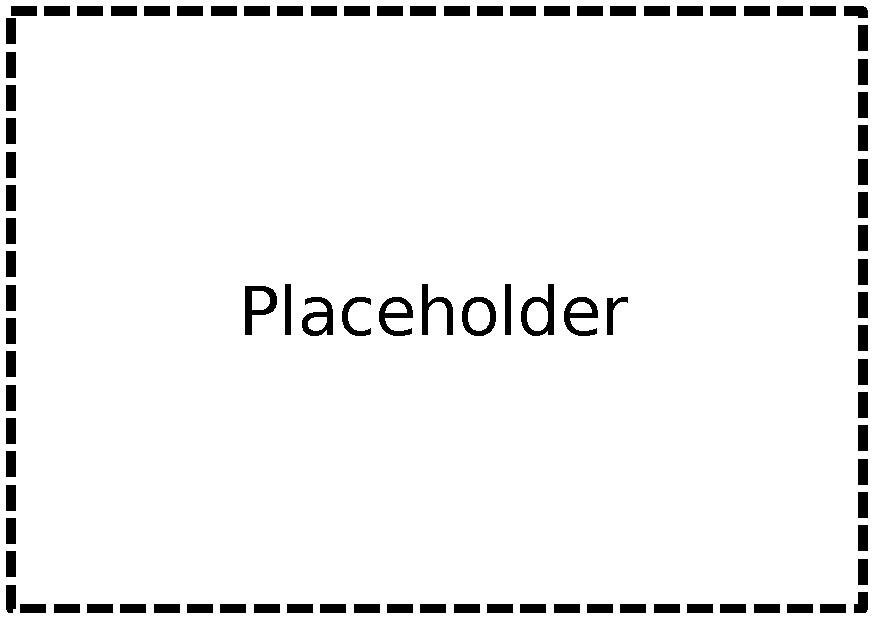
\includegraphics[width=0.5\textwidth]{imgs/lambda-cube.pdf}}
                \caption{Barendregt's "Lambda Cube" \label{fig:lambda-cube}}
            \end{figure}

            %% TODO: introduce logical interpretations for the cube's systems, Martin-Löf, etc.
            %% specially intuitionistic first-order logic for λπ.

        \subsection{Hardware and dependent types}
        \label{sec:hardware-dtp}

            %% TODO
            %% Others
            %% Coquet
            %%     Turning design mistakes into TYPE ERRORS
            %%     Proving properties about circuit behaviour
            %%         Functional correctness in particular.
